\documentclass[a4paper, 10pt]{article}
% [https://github.com/jettan/tikz_cnn]
    \usepackage{graphicx}
    \usepackage{color}
    \usepackage{tikz}
    \usepackage{pgfplots}
    \usepackage{pgf-umlsd}
    \usepackage{ifthen}
    
    \begin{document}
    
    \begin{figure}
        \noindent\resizebox{\textwidth}{!}{
        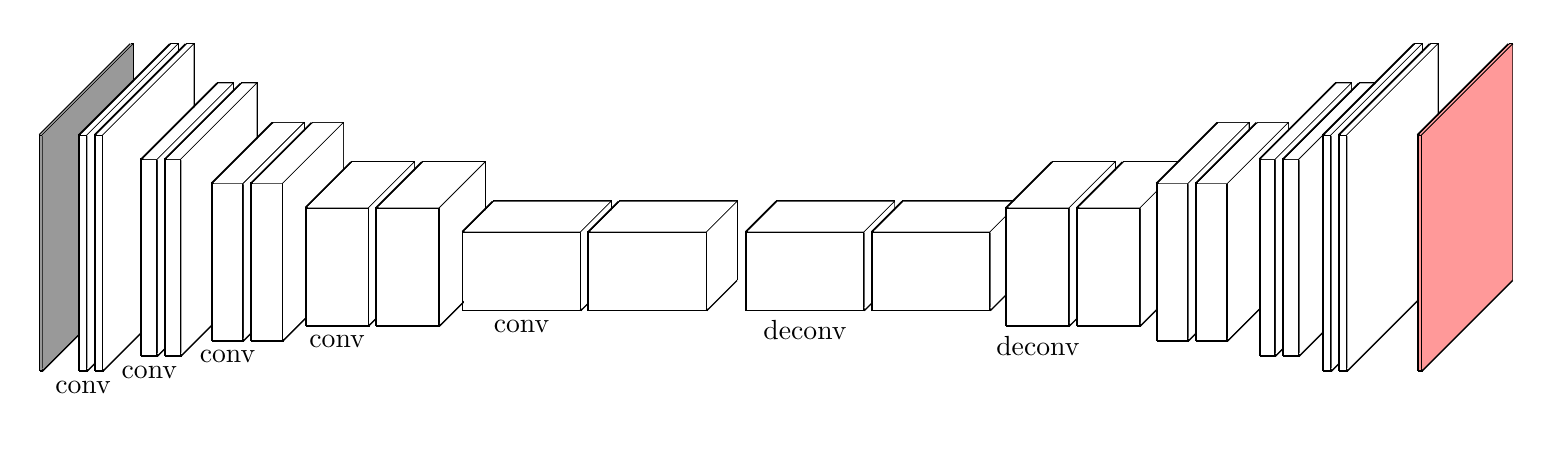
\begin{tikzpicture}
            \draw[use as bounding box, transparent] (-1.8,-1.8) rectangle (17.2, 3.2);
            % \draw[use as bounding box] (-1.8,-1.8) rectangle (17.2, 3.2);
            
    
            % Define the macro.
            % 1st argument: Height and width of the layer rectangle slice.
            % 2nd argument: Depth of the layer slice
            % 3rd argument: X Offset --> use it to offset layers from previously drawn layers.
            % 4th argument: Options for filldraw.
            % 5th argument: Text to be placed below this layer.
            % 6th argument: Y Offset --> Use it when an output needs to be fed to multiple layers that are on the same X offset.
    
            \newcommand{\networkLayer}[6]{
                \def\a{#1} % Used to distinguish input resolution for current layer.
                \def\b{0.02}
                \def\c{#2} % Width of the cube to distinguish number of input channels for current layer.
                \def\t{#3} % X offset for current layer.
                \ifthenelse {\equal{#6} {}} {\def\y{0}} {\def\y{#6}} % Y offset for current layer.
    
                % Draw the layer body.
                \draw[line width=0.25mm](\c+\t,0,0) -- (\c+\t,\a,0) -- (\t,\a,0);                                                      % back plane
                \draw[line width=0.25mm](\t,0,\a) -- (\c+\t,0,\a) node[midway,below] {#5} -- (\c+\t,\a,\a) -- (\t,\a,\a) -- (\t,0,\a); % front plane
                \draw[line width=0.25mm](\c+\t,0,0) -- (\c+\t,0,\a);
                \draw[line width=0.25mm](\c+\t,\a,0) -- (\c+\t,\a,\a);
                \draw[line width=0.25mm](\t,\a,0) -- (\t,\a,\a);
    
                % Recolor visible surfaces
                \filldraw[#4] (\t+\b,\b,\a) -- (\c+\t-\b,\b,\a) -- (\c+\t-\b,\a-\b,\a) -- (\t+\b,\a-\b,\a) -- (\t+\b,\b,\a); % front plane
                \filldraw[#4] (\t+\b,\a,\a-\b) -- (\c+\t-\b,\a,\a-\b) -- (\c+\t-\b,\a,\b) -- (\t+\b,\a,\b);
    
                % Colored slice.
                \ifthenelse {\equal{#4} {}}
                {} % Do not draw colored slice if #4 is blank.
                {\filldraw[#4] (\c+\t,\b,\a-\b) -- (\c+\t,\b,\b) -- (\c+\t,\a-\b,\b) -- (\c+\t,\a-\b,\a-\b);} % Else, draw a colored slice.
            }
    
            % INPUT
            \networkLayer{3.0}{0.03}{-0.5}{color=gray!80}{}
    
            % ENCODER
            \networkLayer{3.0}{0.1}{0.0}{color=white}{conv}{}    % S1
            \networkLayer{3.0}{0.1}{0.2}{color=white}{}{}        % S2
            \networkLayer{2.5}{0.2}{0.6}{color=white}{conv}{}    % S1
            \networkLayer{2.5}{0.2}{0.9}{color=white}{}{}        % S2
            \networkLayer{2.0}{0.4}{1.3}{color=white}{conv}{}    % S1
            \networkLayer{2.0}{0.4}{1.8}{color=white}{}{}        % S2
            \networkLayer{1.5}{0.8}{2.3}{color=white}{conv}{}    % S1
            \networkLayer{1.5}{0.8}{3.2}{color=white}{}{}        % S2
            \networkLayer{1.0}{1.5}{4.1}{color=white}{conv}{}    % S1
            \networkLayer{1.0}{1.5}{5.7}{color=white}{}{}        % S2
    
            % DECODER
            \networkLayer{1.0}{1.5}{7.7}{color=white}{deconv}{}   % S1
            \networkLayer{1.0}{1.5}{9.3}{color=white}{}{}         % S2
            \networkLayer{1.5}{0.8}{11.2}{color=white}{deconv}{}  % S1
            \networkLayer{1.5}{0.8}{12.1}{color=white}{}{}        % S2
            \networkLayer{2.0}{0.4}{13.3}{color=white}{}{}        % S1
            \networkLayer{2.0}{0.4}{13.8}{color=white}{}{}        % S2
            \networkLayer{2.5}{0.2}{14.8}{color=white}{}{}        % S1
            \networkLayer{2.5}{0.2}{15.1}{color=white}{}{}        % S2
            \networkLayer{3.0}{0.1}{15.8}{color=white}{}{}        % S1
            \networkLayer{3.0}{0.1}{16}{color=white}{}{}          % S2
    
            % OUTPUT
            \networkLayer{3.0}{0.05}{17}{color=red!40}{}{}          % Pixelwise segmentation with classes.
    
    
        \end{tikzpicture}
        }
        \caption{Example CNN.}
        \label{fig:cnn}
    \end{figure}
    
    \end{document}